\documentclass[a4paper,12pt]{article}
\usepackage{graphicx}
\usepackage[left=30mm, right=30mm, top=30mm, bottom=35mm]{geometry}
\usepackage{amsmath}
\usepackage{siunitx}
\usepackage{fancyhdr}
\usepackage{url}
\pagestyle{fancy}
%-------------------------------------------------------------------------------
\lhead{\textbf{Spring 2019}}
\rhead{\textbf{CE394M Advanced Analysis in Geotechnical Engineering}}
\cfoot{\thepage}
%-------------------------------------------------------------------------------

\begin{document}
\begin{centering}
	\textbf{
		Assignment 4: FEM: Isoparametric elements, Gauss integration and solvers\\
		Assigned: 25th February 2019\\
		Due: 8th March 2019\\
	}
\end{centering}

\vspace{1em}
 
\begin{enumerate}

	\item For the six noded-triangle shown. The nodal temperatures are $T^e = \begin{bmatrix}300 & 0 & 0 & 0 & 340 & 0 \end{bmatrix}^T$. Compute the temperature and its gradient at the point $P$ with the coordinates $x = 1.5$ and $y = 2.0$.

		
		\begin{figure}[!h]
			\centering
			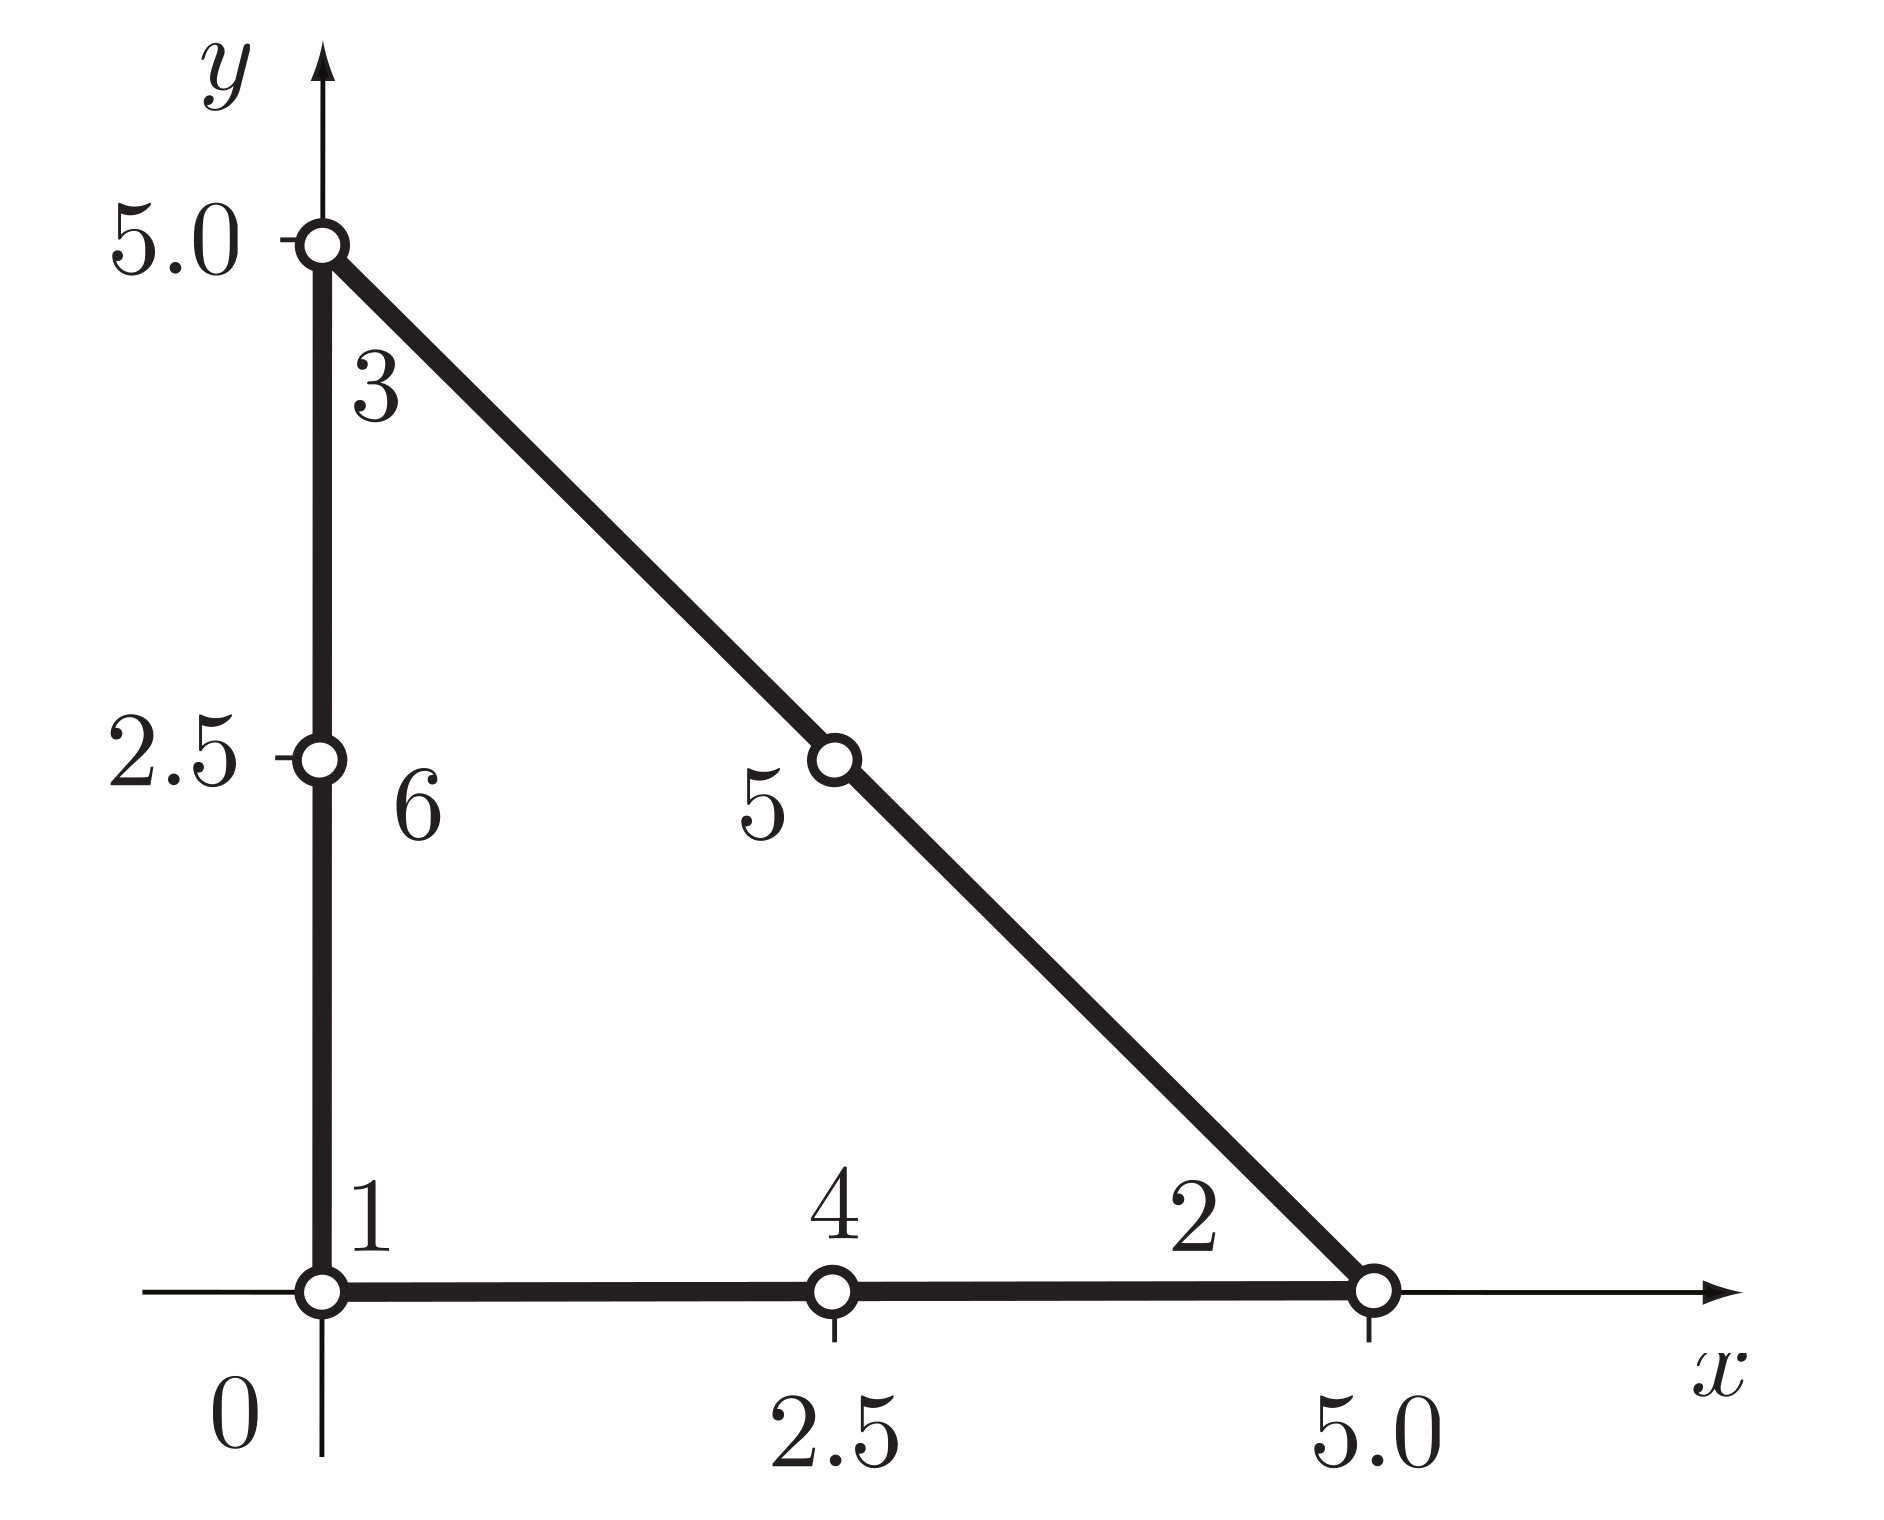
\includegraphics[width=0.5\textwidth]{figs/6noded-triangle.png}
		\end{figure}

	Use the isoparametric shape functions provided in the data sheet.
	
	
	\item For the isoparametric mapping shown below
		\begin{enumerate}
			\item Compute the $x$ and $y$ coordinates of the point $\xi = 0.5$, $\eta = 0.5$ in the physical domain.
			\item Compute $\frac{\partial N_1}{\partial x}$ for the same point.
		\end{enumerate}
		
		\begin{figure}[!h]
			\centering
			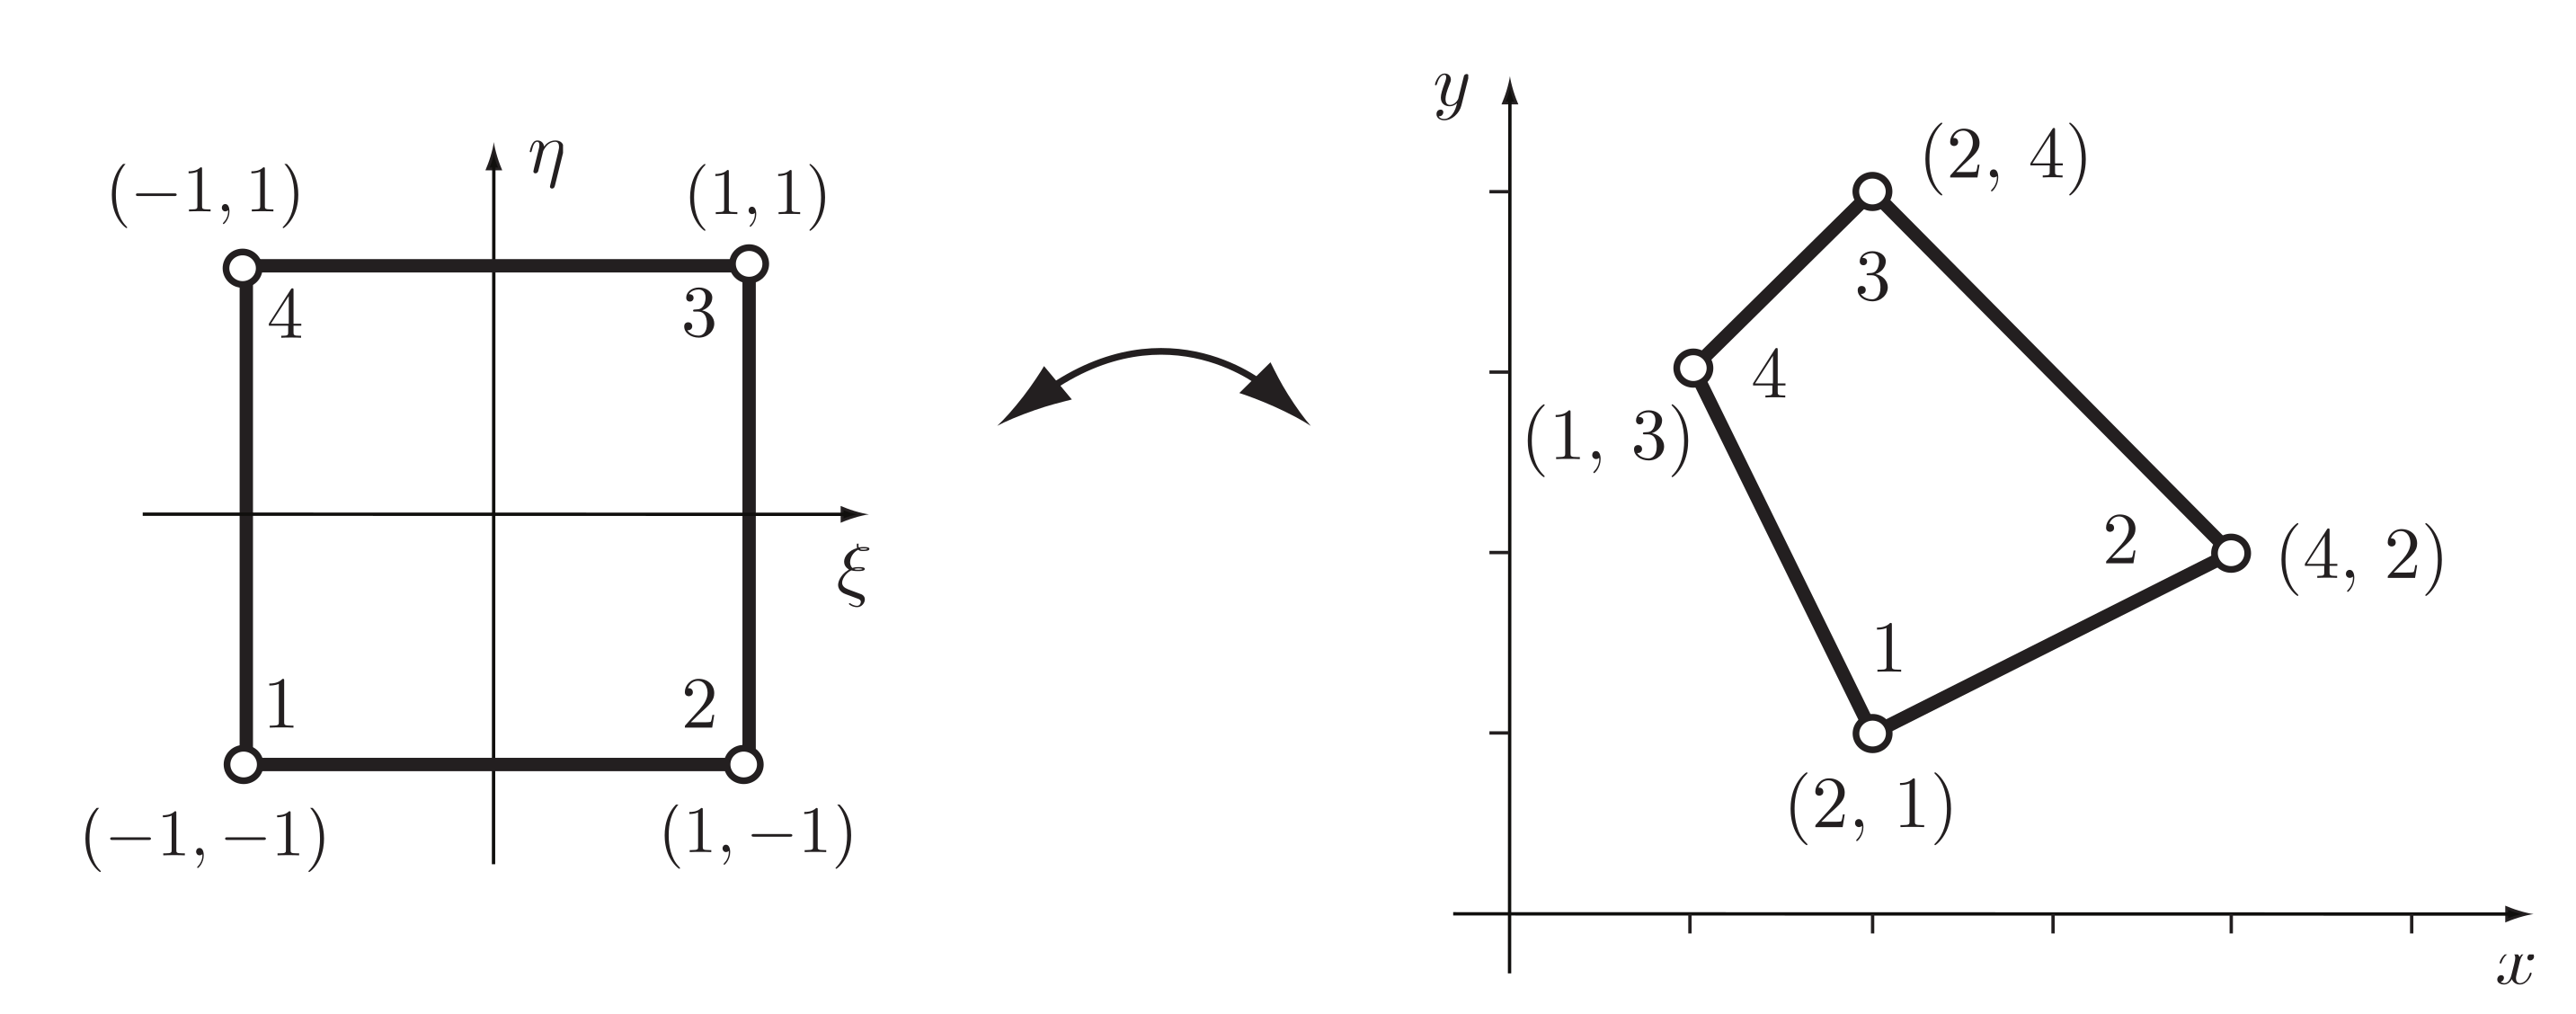
\includegraphics[width=\textwidth]{figs/isoparametric-mapping.png}
		\end{figure}
	
	\item Evaluate the following three integrals using one, two and three-point Gauss integration.
	Compare your results with the results of analytic integration.
		\begin{enumerate}
			\item $\int_{-1}^{+1}(3\xi^2 + 2\xi) d\xi$
			\item $\int_{-1}^{+1} \cos \xi d\xi$
			\item $\int_{0}^{3} (3x^2 + x) dx$
		\end{enumerate}
		
	\item Consider the following quadrilateral mesh, sketch (1D is fine) the temperature distribution across the mesh assuming a hear source on the left boundary of the mesh and comment on the suitability of the mesh for finite element computation and the need for the transition element (element \#2)?
				
		\begin{figure}[!h]
			\centering
			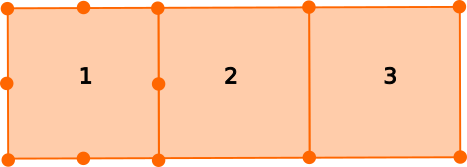
\includegraphics[width=0.7\textwidth]{figs/transition-elements.png}
		\end{figure}

	\item Develop a Python script for the Newton Raphson method to solve non-linear force-displacement relationships. Test and comment on the accuracy and efficiency of the NR to solve: $f = - 2 u^2 + 2 u$, where $u$ denotes the displacement and $f$ refers to the internal force. For the analytical solution plot the displacement $u$ between 0 and 1.
\end{enumerate}

\section*{Datasheet}
The shape functions for a 6-noded triangle element are:
\begin{align*}
N_1 & = 2(1-\xi -\eta)^2 - (1 -\xi -\eta)\\
N_2 & = 2\xi^2 -\xi\\
N_3 & = 2\eta^2 -\eta\\
N_4 & = 4\xi(1 - \xi - \eta)\\
N_5 & = 4\xi\eta \\
N_6 & = 4 \eta(1 - \xi - \eta)\\
\end{align*}

\end{document}

